% !TEX root = ../dissertacao.tex
\chapter{Introdução}
\label{cap:introducao}
    % evolução da tecnologia -> transistores menores
    % circuitos modernos muito grande grandes -> ferramentas de EDA
    % eletrônica de consumo -> tempo limitado para projeto de um circuito
    % é benéfico a redução de tempo na execução dos algoritmos sem perda da qualidade da solução
    % memória representa gargalo -> explorar a localidade na cache
    %
    % uma possível solução que não altera a qualidade da solução é o melhor armazenamento dos dados

A evolução da tecnologia de fabricação de \acp{ic} vem permitindo uma redução drástica e contínua das dimensões dos transistores.
O consequente aumento de densidade permitiu que atualmente sejam fabricados \acp{ic} com dezenas de milhões de transistores.
Além deste número elevado de elementos, os circuitos contemporâneos devem respeitar uma ampla gama de restrições, sejam elas de atraso, potência e\@/\@ou área.
Adicionalmente, o prazo entre o projeto e a fabricação de um chip é cada vez mais limitado para que um novo produto eletrônico possa garantir o mercado (\textit{time-to-market})~\cite{papa2011physical}.
Neste contexto, é mandatório o uso de Ferramentas de \ac{eda} no projeto de \acp{ic} contemporâneos.
% Portanto, as Ferramentas de \ac{eda} são obrigatórias no design de \acp{ic} modernos.

% Ferramentas de \ac{eda} para o projeto de circuitos digitais seguem uma metodologia de projeto denominada \textit{standard cell}.
O fluxo de projeto com ferramentas de \ac{eda} segue a metodologia denominada \textit{standard cell}.
Esta metodologia se caracteriza pela adoção de bibliotecas de células padrão pré-projetadas e pré-caracterizadas, que descrevem as informações lógicas, físicas e elétricas dos elementos combinacionais e sequenciais a serem utilizados na síntese~\cite{kahng2011vlsi}.

Um fluxo de projeto que segue a metodologia \textit{standard cell} é tipicamente dividido em diversas etapas.
A Figura~\ref{fig:exemplo_fluxo} apresenta as principais etapas deste fluxo, onde cada etapa pode ser subdividida em outras.
Este fluxo inicia com a captura do comportamento do sistema, em um alto nível de abstração (especificação do sistema).
Após, o sistema é particionado em \textit{software} e \textit{hardware} e a arquitetura da parte de \textit{hardware} é definida (projeto arquitetural).
A seguir, é criada a descrição no \ac{rtl}, usando uma \ac{hdl}, tal como VHDL e Verilog (projeto funcional e lógico).
Tal descrição é traduzida para o nível lógico (síntese lógica), originando uma lista de portas lógicas, elementos sequenciais (\textit{latches} e\@/\@ou \textit{flip-flops}) e interconexões, geralmente referenciada por \textit{netlist}.

\begin{figure}[]
    \centering
    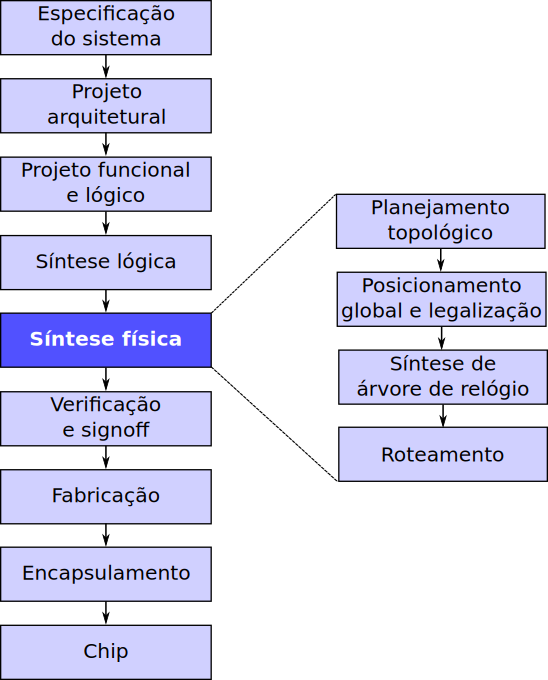
\includegraphics[width=0.5\textwidth]{img/introducao/exemplo_fluxo.pdf}
    \caption[Etapas do fluxo \textit{standard cell}.]{Exemplo das etapas de um fluxo de projeto com metodologia \textit{standard cell}. Figura adaptada de~\citeonline{kahng2011vlsi}.}
    \label{fig:exemplo_fluxo}
\end{figure}

Na etapa de síntese física as portas lógicas e os elementos sequenciais da \textit{netlist} são associados a descrições geométricas de associações de transistores referenciadas por "células", as quais estão disponíveis na \textit{standard cells}.
Após, as células são posicionadas e interconectadas, formando uma descrição completa das máscaras que serão usadas na fabricação do \ac{ic}.
Tal descrição ainda deve ser verificada antes de ser enviada para a fabricação (verificação e signoff).
A verificação é realizada seguindo regras que representam as limitações físicas do meio de fabricação.
Por exemplo, todos os fios devem estar a uma distância mínima e ter uma determinada largura mínima.
Uma vez fabricado, o \ac{ic} é testado e empacotado (etapa de encapsulamento).

Observe que a Figura~\ref{fig:exemplo_fluxo} apresenta um modelo simplificado do fluxo executado no projeto de um \ac{ic} real.
% Caso a Figura~\ref{fig:exemplo_fluxo} apresentasse o fluxo completo, seria necessário inserir diversas etapas de otimização, bem como caminhos que regressam no fluxo.
Note que este não é um fluxo linear, mas iterativo, onde pode ser necessário voltar para etapas anteriores do fluxo.
Por exemplo, caso ocorra um congestionamento numa determinada área do circuito, o roteamento do circuito pode se tornar impossível de ser realizado. Neste caso, o projeto deve retornar à etapa de posicionamento e legalização das células.

Ao mesmo tempo que cada etapa do fluxo \textit{standard cell} apresenta grande complexidade, segundo~\citeonline{papa2011physical}, é desejável que o fluxo completo de projeto seja realizado em um curto período de tempo (12 horas no processo da IBM). Logo, é essencial que cada etapa seja executada no menor tempo possível, o que demanda a exploração de diversas técnicas para redução de tempo de execução.
Portanto, as ferramentas de \ac{eda} devem tratar um grande volume de dados em um curto período de tempo.
Para isso, estas ferramentas devem empregar otimizações de software, como o uso de melhores estruturas de dados, paralelização e exploração da localidade de dados na cache.


% Diversos trabalhos na literatura buscam otimizar o tempo de execuções de aplicações.
% \citeonline{majeti2013compiler} utilizou heurísticas e metadados inseridos no código fonte para, em tempo de compilação, selecionar as estrutura de dados para execução em CPU\@/\@GPU.
% Já \citeonline{sung2010data} realizaram conversões das estruturas de dados para aumentar a utilização da cache compartilhada empregando transformações em tempo de compilação.
% Porém, a grande maioria destes trabalhos realizam as otimizações com foco em uma única arquitetura, avaliam seus resultados com \textit{benchmarks} sintéticos e nenhum destes trabalhos foi avaliado no contexto de \textit{Physical Design}.

% Outra adversidade que as ferramentas de \ac{eda} enfrentam é como modelar os dados para que as diversas relações do fluxo do projeto seja suportadas.
% Modelando com modelos tradicionais de programação, como \ac{ood}, a hierarquia das classes pode forçar a repetição de código e\@/\@ou a utilização de herança múltipla para um determinado problema.
% Herança múltipla não é suportada por todas as linguagens de programação e, mesmo quando suportada, não é recomendável porque pode levar a uma codificação confusa que dificultaria a manutenção do código~\cite{nystrom2014game}.

Este trabalho irá focar na exploração da localidade da cache no contexto de ferramentas de Physical Design.
Para aumentar a localidade da cache, este trabalho irá aplicar otimizações previamente ao código ser compilado.
Para realizar estas otimizações, primeiro serão identificadas as características de cada algoritmo e sobre quais dados este irá operar.
Posteriormente, será otimizada a organização destes dados de forma a maximizar a utilização dos dados recuperados pela cache.
Por fim, este trabalho ira comparar a abordagem tradicional (orientada a objetos) com a abordagem otimizada considerando o número total de \textit{cache misses} e o tempo de execução. Informações pertinentes a arquiteturas de cache (tamanho de blocos e número de níveis) não serão consideradas no momento da organização dos dados.
Estas informações não serão consideradas pois a organização dos dados deve suportar diversas arquiteturas de cache.


\section{Justificativa}

    Apesar de vários trabalhos encontrados na literatura fazerem otimizações de software mencionadas na seção anterior, nenhum deles avalia o impacto destas diferentes estratégias quando aplicadas no contexto de Physical Design.

    % Portanto, é desejável uma análise quantitativa do impacto da organização dos dados no contexto de Physical Design, sobretudo, com uma comparação que faça uso de uma infraestrutura realista e bem consolidada na academia.
    Portanto, é desejável uma análise quantitativa do impacto da organização dos dados no contexto de Physical Design, sobretudo, com um estudo de problemas reais utilizando entradas realistas para a experimentação.

\section{Objetivos e Contribuições Pretendidas}

    Este trabalho tem como objetivo a avaliação quantitativa do impacto causado pela organização dos dados em diferentes algoritmos no contexto de Physical Design.

    Os objetivos específicos deste trabalho são:

    \begin{itemize}
        \item Implementar três algoritmos de Physical Design com diferentes tipos de organização dos dados;
        \item Avaliar as organizações dos dados propostas comparando-as com a modelagem tradicional utilizada, resultante do uso de orientação a objetos. A comparação é realizada comparando o número de \textit{cache misses} gerados pelas algoritmos, bem como o tempo de execução;
        \item Avaliar a facilidade e o desempenho da paralelização dos algoritmos implementados com as diferentes organização dos dados.
    \end{itemize}

    Cumprindo estes objetivos, espera-se alcançar as seguintes contribuições científicas e tecnológicas:

    \begin{itemize}
        \item Implementação de um sistema de componentes e entidades;
        \item Avaliação quantitativa do desempenho causado pela modelagem dos dados em três algoritmos da síntese física;
        \item Resultados experimentais utilizando uma infraestrutura baseada em circuitos industriais;
        \item Resultados experimentais analisando problemas reais com dados realistas. Como dados de entrada serão utilizados circuitos industriais oriundos da competição ICCAD CAD Context 2015~\cite{kim2015}.
    \end{itemize}


% \section{Metodologia}
%         Implementar versões de problemas
%         avaliar quantitativamente o número de cache misses
%         avaliar quantitativamente o tempo de execução
%
% \section{Limitações(escopo) deste trabalho}
%         somente 3 problemas avaliados
%         somente uma arquitetura de processador e cache
%         paralelização com um chunk único

% \section{Organização deste trabalho}
\section{Organização deste texto}

O Capítulo~\ref{cap:trabalhos_correlatos} apresenta os trabalhos correlatos na otimização da organização dos dados para uma melhor utilização da cache.
No Capítulo~\ref{cap:tecnica_proposta} é apresentada a proposta de organização dos dados e os possíveis impactos causados pelas mesmas segundo o contexto de Physical Design.
O Capítulo~\ref{cap:resultados} apresenta os resultados preliminares já obtidos até o presente momento da escrita deste documento.
O Capítulo~\ref{cap:cronograma} descreve as atividades já realizadas e as que ainda precisam serem realizadas para a conclusão deste mestrado. Neste capítulo também é apresentado o cronograma que demonstra que este mestrado será concluído dentro do prazo disposto.
